\chapter{Симметричные квазиньютоновские обновления с контролем секущих условий}\label{ch:symmetric}

\section{Мотивация}\label{sec:ss_motivation}

В предыдущих разделах метод SP-Broyden решил задачу сохранения секущих
условий для общих систем $F(x) = 0$, однако матрица $B_k$ при этом
несимметрична. Для задач безусловной оптимизации, где $F = \nabla f$ и
$J^* = \nabla^2 f(x^*)$ симметричен, естественно требовать $B_k = B_k^\top$.

Классические симметричные квазиньютоновские обновления~---
SR1 (\emph{symmetric rank-one}, Дэвидон~\cite{davidon1991}) и~PSB
(\emph{Powell symmetric Broyden}, Пауэлл~\cite{powell1970})~---
удовлетворяют текущему секущему условию $B_{k+1} s_k = y_k$,
но не контролируют невязку прошлых секущих
$R_{\mathrm{past}} = B_k S_{\mathrm{past}} - Y_{\mathrm{past}}$.
Следующая теорема показывает, что одновременное точное выполнение
всех секущих и симметрии невозможно.

\begin{theorem}[Несовместность симметрии и одновременного сохранения всех секущих]\label{thm:incompat}
Пусть $B_k\in\RR^{n\times n}$ удовлетворяет всем прошлым секущим
условиям $B_k s_j = y_j$ ($j=0,\dots,k-1$), и пусть симметричное
обновление $B_{k+1} = B_k + \Delta B$, $\Delta B = \Delta B^\top$,
сохраняет все секущие до~$k$-й включительно:
\[
  B_{k+1} s_j = y_j \;\;(j = 0,\dots,k-1),
  \qquad B_{k+1} s_k = y_k.
\]
В~терминах поправки $\Delta B$ это означает
\[
  \Delta B\, s_j = 0 \;\;(j=0,\dots,k-1),
  \qquad \Delta B\, s_k = r_k,
  \qquad r_k := y_k - B_k s_k.
\]
Тогда остаток $r_k$ обязан быть ортогонален всем прошлым шагам:
\begin{equation}\label{eq:incompat}
  s_j^\top r_k = 0 \qquad \forall\, j < k.
\end{equation}
\end{theorem}

\begin{proof}
Для произвольного $j < k$:
\begin{equation}\label{eq:incompat-chain}
  s_j^\top r_k
  \;\stackrel{(1)}{=}\; s_j^\top (\Delta B\, s_k)
  \;\stackrel{(2)}{=}\; s_j^\top \Delta B^\top s_k
  \;\stackrel{(3)}{=}\; (\Delta B\, s_j)^\top s_k
  \;\stackrel{(4)}{=}\; 0,
\end{equation}
где~(1)~--- текущее секущее условие $\Delta B\, s_k = r_k$;
(2)~--- симметрия $\Delta B = \Delta B^\top$;
(3)~--- тождество $u^\top A^\top v = (A u)^\top v$;
(4)~--- сохранение $j$-й прошлой секущей $\Delta B\, s_j = 0$.
\end{proof}

\begin{remark}[Когда условие~\eqref{eq:incompat} выполнено]
Пусть $F = \nabla f$, $f\in C^2$. По~интегральной форме теоремы
о~среднем для градиента
\[
  y_j \;=\; \nabla f(x_j + s_j) - \nabla f(x_j) \;=\; \bar{H}_j\, s_j,
  \qquad
  \bar{H}_j \;:=\; \int_0^1 \nabla^2 f(x_j + t\, s_j)\, dt,
\]
где $\bar{H}_j$~--- средний гессиан вдоль $j$-го шага (симметричен).
Если $B_k$ симметричен и удерживает прошлые секущие $B_k s_j = y_j$,
то $s_j^\top B_k = (B_k s_j)^\top = (\bar{H}_j s_j)^\top = s_j^\top \bar{H}_j$,
и левая часть~\eqref{eq:incompat} принимает вид
\begin{equation}\label{eq:incompat-hessian}
  s_j^\top r_k
  \;=\; s_j^\top y_k - s_j^\top B_k s_k
  \;=\; s_j^\top \bar{H}_k s_k - s_j^\top \bar{H}_j s_k
  \;=\; s_j^\top (\bar{H}_k - \bar{H}_j)\, s_k.
\end{equation}

\emph{Случай квадратичной $f$.} Если $f(x) = \tfrac12 x^\top A x + b^\top x + c$,
то $\nabla^2 f \equiv A$, и потому $\bar{H}_k = \bar{H}_j = A$ для любых $j,k$.
Правая часть~\eqref{eq:incompat-hessian} обращается в~нуль тождественно,
условие~\eqref{eq:incompat} выполнено автоматически~--- симметричное
обновление, одновременно удерживающее все секущие, существует
(и~это $\Delta B$, восстанавливающая $A$).

\emph{Случай неквадратичной $f$.} Если $\nabla^2 f$~--- не~константа, то
$\bar{H}_k - \bar{H}_j$ зависит от~траектории и~ненулева в~общем положении;
разность исчезает лишь асимптотически, $x_k, x_j \to x^*$, по~непрерывности
гессиана. Поэтому в~произвольной конечной окрестности
условие~\eqref{eq:incompat} не~выполнено~--- симметричного обновления,
точно удерживающего все секущие, в~общем случае \emph{не существует}.
Это и~есть та~жёсткость, которую в~\S\ref{sec:ss_construction}
снимает~SS-конструкция: вместо точного удержания прошлых секущих
минимизируется их~остаток в~ортогональном к~$s_k$ дополнении.
\end{remark}


% ============================================================
\section{Конструкция и алгоритм SS-\texorpdfstring{$\mathcal{U}$}{U}}
\label{sec:ss_construction}

\begin{definition}[Секантно-стабилизированное обновление]
\label{def:ss}
Пусть $\mathcal{U}$~--- базовое симметричное квазиньютоновское
обновление, удовлетворяющее текущему секущему условию
$\mathcal{U}(B_k, s_k, y_k)\, s_k = y_k$.
\emph{Секантно-стабилизированное расширение}
$\mathrm{SS}\text{-}\mathcal{U}$:
\begin{equation}\label{eq:ss_update}
  B_{k+1} = \underbrace{\mathcal{U}(B_k, s_k, y_k)}_{\displaystyle B'_k}
  + \sigma_k^*\, u_k^*\, u_k^{*\top},
  \qquad u_k^* \perp s_k,\;\; \|u_k^*\| = 1,
\end{equation}
где $u_k^*$~--- ведущий собственный вектор матрицы
$P_k M'_k P_k$,
\[
  M'_k = \tfrac{1}{2}(R'_k S_p^\top + S_p R_k^{\prime\top}),
  \qquad
  R'_k = B'_k S_p - Y_p,
  \qquad
  P_k = I - \hat{s}_k \hat{s}_k^\top,
\]
а~$\sigma_k^*$ выбирается из минимума $\|R'_k + \sigma\, u^*\, u^{*\top} S_p\|_F^2$:
\begin{equation}\label{eq:ss_sigma}
  \sigma_k^* = -\frac{u_k^{*\top} R'_k S_p^\top u_k^*}
                     {\|S_p^\top u_k^*\|^2}.
\end{equation}
\end{definition}

\begin{lemma}[Вариационная характеристика SS-$\mathcal{U}$-коррекции]
\label{lem:ss_variational}
Пусть $R'_k = B'_k S_p - Y_p$, $M'_k = \tfrac{1}{2}(R'_k S_p^\top + S_p R_k^{\prime\top})$
и пара $(\sigma_k^*, u_k^*)$ доставляет минимум функционалу
$\Phi(\sigma, u) = \|R'_k + \sigma\, u u^\top S_p\|_F^2$ при ограничениях
$\|u\|=1$, $u\perp s_k$. Тогда:
\begin{enumerate}
  \item для каждого допустимого~$u$ оптимальное~$\sigma$ равно
    $\sigma_k^*(u) = -(u^\top M'_k u)/\|S_p^\top u\|^2$, и подстановка даёт
    \begin{equation}\label{eq:ss_phi_min_sigma}
      \min_\sigma \Phi(\sigma, u)
      \;=\; \|R'_k\|_F^2 \;-\; \frac{(u^\top M'_k u)^2}{\|S_p^\top u\|^2};
    \end{equation}
  \item оптимальный $u_k^*$~--- ведущий по модулю обобщённый собственный
    вектор пары $(M'_k,\, S_p S_p^\top)$ на $s_k^\perp$:
    $M'_k u_k^* = \lambda^*\, S_p S_p^\top u_k^*$, $u_k^*\perp s_k$,
    $\|u_k^*\|=1$ с максимальным $|\lambda^*|$.
\end{enumerate}
\end{lemma}

\begin{proof}
Раскрытие $\|R'_k + \sigma uu^\top S_p\|_F^2$ через
$\|A+B\|_F^2 = \|A\|_F^2 + 2\,\mathrm{tr}(A^\top B) + \|B\|_F^2$ даёт
\[
  \Phi(\sigma, u)
  = \|R'_k\|_F^2 + 2\sigma\,\mathrm{tr}(R_k^{\prime\top} u u^\top S_p)
                + \sigma^2\,\|u u^\top S_p\|_F^2.
\]
Сворачивая след $\mathrm{tr}(R_k^{\prime\top} u u^\top S_p) = u^\top S_p R_k^{\prime\top} u = u^\top M'_k u$
(в последнем равенстве учтено, что $u^\top R'_k S_p^\top u = u^\top S_p R_k^{\prime\top} u$ как
скаляры; их полусумма~--- $u^\top M'_k u$) и
$\|u u^\top S_p\|_F^2 = \|u\|^2\|S_p^\top u\|^2 = \|S_p^\top u\|^2$ при $\|u\|=1$:
\begin{equation}\label{eq:ss_phi_quad}
  \Phi(\sigma, u)
  = \|R'_k\|_F^2 + 2\sigma\,(u^\top M'_k u) + \sigma^2\,\|S_p^\top u\|^2.
\end{equation}
Минимум по~$\sigma$ при фиксированном~$u$ достигается в стационарной точке
$\partial_\sigma \Phi = 0$, откуда~(п.~1).
Подставляя в~\eqref{eq:ss_phi_quad}, получаем
$\Phi(\sigma_k^*(u), u) = \|R'_k\|_F^2 - (u^\top M'_k u)^2/\|S_p^\top u\|^2$,
и минимум по~$u$ эквивалентен максимуму обобщённого Rayleigh-частного
$\rho(u) = (u^\top M'_k u)^2/\|S_p^\top u\|^2$ на $s_k^\perp \cap S^{n-1}$.
Стационарные точки $\rho$ удовлетворяют обобщённой собственной задаче
$M'_k u = \lambda\, S_p S_p^\top u$, $u\perp s_k$~(п.~2).
\end{proof}

\begin{remark}[Связь с реализацией Алгоритма~\ref{alg:ss_u}]
\label{rem:ss_variational_alg}
Лемма~\ref{lem:ss_variational} формализует точную вариационную задачу
для пары $(\sigma_k^*, u_k^*)$. В реализации (Алгоритм~\ref{alg:ss_u},
Шаги~3--4) используется упрощение: $u_k^*$ берётся как ведущий
\emph{обычный} собственный вектор $P_k M'_k P_k$ на $s_k^\perp$, что
соответствует замене знаменателя $\|S_p^\top u\|^2$ на $\|u\|^2 = 1$
в~\eqref{eq:ss_phi_min_sigma}. Эта замена эквивалентна предположению, что
$\|S_p^\top u\|$ слабо зависит от~$u$ среди допустимых направлений; при
адаптивном порожнии $\sigma_{\min}(\widehat S_p) \ge \sigma_0$ (\S\ref{sec:ss_construction}),
гарантируемом safeguard'ом $\varepsilon_S$ на знаменатель~\eqref{eq:ss_sigma},
обе задачи имеют общий ведущий собственный вектор с точностью
$\mathcal{O}(\kappa(S_p))$. Безусловное~$\sigma_k^*$ из~\eqref{eq:ss_sigma}
вычисляется в Алгоритме~\ref{alg:ss_u} по точной формуле п.~1
(шаг $\sigma_k^* \leftarrow -(u^\top R'_k\,\eta)/\|\eta\|^2$).
\end{remark}

\paragraph{Базовые обновления $\mathcal{U}$.}
Алгоритм~SS-$\mathcal{U}$, приведённый ниже, не~зависит от~выбора
$\mathcal{U}$, кроме явного вычисления $B'_k=\mathcal{U}(B_k,s_k,y_k)$
на~Шаге~1. В~численных экспериментах настоящей главы рассматриваются
два классических индефинитных симметричных обновления:
\[
  \mathcal{U}_{\mathrm{SR1}}(B,s,y)
   \;=\; B + \frac{r r^\top}{r^\top s},
  \qquad
  \mathcal{U}_{\mathrm{PSB}}(B,s,y)
   \;=\; B + \frac{r s^\top + s r^\top}{s^\top s}
        - \frac{(s^\top r)\, s s^\top}{(s^\top s)^2},
  \qquad r = y - Bs.
\]
SR1 требует skip-rule~\cite[\S 6.2]{bfgs}: при
$|s^\top r|<\varepsilon_{\mathrm{skip}}\Norm{s}\Norm{r}$
обновление пропускается, $B'_k = B_k$. PSB skip-правил не~требует.
SS-расширение строится по~единому шаблону~\eqref{eq:ss_update},
ниже~--- общий псевдокод.

\medskip
Реализация~\eqref{eq:ss_update} вносит две численные проверки на
стороне MS-коррекции~--- вырождение $u_k^*$ после репроекции
на~$s_k^\perp$ (порог $\varepsilon_u$) и устойчивость знаменателя
$\sigma_k^*$ (порог $\varepsilon_S$); конкретное базовое $\mathcal{U}$
может вносить свой safeguard (skip-rule для $\mathcal{U}=\mathrm{SR1}$).
Ключевое наблюдение для Шага~3:
$M'_k=\tfrac12(R'_k S_p^\top+S_p R_k^{\prime\top})$~--- сумма двух
матриц ранга $\le p+1$, поэтому
\begin{equation}\label{eq:ss_low_rank}
  \mathrm{rank}(P_k M'_k P_k)
   \;\le\; \mathrm{rank}(M'_k)
   \;\le\; 2(p+1),
\end{equation}
и весь ненулевой спектр $A_k=P_k M'_k P_k$ лежит
в~$\mathrm{range}(P_k[S_p,R'_k])$. Собственная задача переносится
из~$\RR^n$ в~подпространство размерности $r\le 2(p+1)$ через
QR-ортогонализацию этого базиса (приём, стандартный для блочных
Ланцош-итераций~\cite[Гл.~13]{parlett1998}; ср.\ также подход
Fang--Saad~\cite{fang2009} для мультисекантных схем).
Алгоритм~\ref{alg:ss_u} непосредственно реализует эту редукцию;
эквивалентность с~прямой формой $\mathtt{eigh}(A_k)$ и~детализация
стоимости~--- в~Замечании~\ref{rem:ss_u_cost}.

\begin{breakablealgorithm}
\caption{SS-$\mathcal{U}$\ $(\nabla f,\,x_0,\,p_{\max},\,\varepsilon;\,
        \mathcal{U},\,\varepsilon_u,\,\varepsilon_S)$}
\label{alg:ss_u}
\begin{algorithmic}
\Require $\nabla f\colon\RR^n\to\RR^n$,\ $x_0\in\RR^n$,\
         $p_{\max}\ge 0$,\ $\varepsilon>0$
\Require базовое симметричное обновление $\mathcal{U}(B,s,y)$
         (например, $\mathcal{U}_{\mathrm{SR1}}$ со~skip-rule
         или $\mathcal{U}_{\mathrm{PSB}}$)
\Require \emph{(численные пороги MS-коррекции; стандартные значения)}\hfil\null
         \par\hangindent=2em
         $\varepsilon_u=10^{-12}$ (невырожденность $u_k^*$ после репроекции
         на~$s_k^\perp$),\
         $\varepsilon_S=10^{-15}$ (нижний порог $\Norm{S_p^{\top} u_k^*}^2$
         в~знаменателе~\eqref{eq:ss_sigma}).
\State $B_0 \leftarrow I_n$,\quad $k \leftarrow 0$
\While{$\Norm{\nabla f(x_k)}\ge \varepsilon$}
  \State Решить $B_k\,d_k = -\nabla f(x_k)$
  \State $\alpha_k \leftarrow$ Armijo-backtracking на $f$
       (Алгоритм~\ref{alg:qn_armijo}, $\phi = f$,
        \S\ref{sec:globalization})
  \State $x_{k+1}\leftarrow x_k+\alpha_k d_k$,\
         $s_k\leftarrow \alpha_k d_k$,\
         $y_k\leftarrow \nabla f(x_{k+1})-\nabla f(x_k)$
  %---- Шаг 1. Базовое обновление U ----
  \State $B'_k \leftarrow \mathcal{U}(B_k, s_k, y_k)$
       \Comment{$B'_k = B_k$, если $\mathcal{U}$ срабатывает skip-rule}
  %---- Шаг 2. Окно прошлых секущих ----
  \State $p \leftarrow \min(p_{\max},k)$
  \State $S_p\leftarrow [s_k\mid s_{k-1}\mid\cdots\mid s_{k-p}]$,\quad
         $Y_p\leftarrow [y_k\mid y_{k-1}\mid\cdots\mid y_{k-p}]$
       \hfill\Comment{$n\times(p{+}1)$}
  %---- Шаг 3. Ведущий собств. вектор $P_k M'_k P_k$ через редукцию ----
  \If{$p\ge 0$ \textbf{and} $S_p$ непуста}
    \State $R'_k \leftarrow B'_k S_p - Y_p$
       \hfill\Comment{$n\times(p{+}1)$,\ $O(n^2 p)$}
    \State $\hat s_k \leftarrow s_k/\Norm{s_k}$
    \State $W \leftarrow [S_p\mid R'_k] - \hat s_k\bigl(\hat s_k^{\top}[S_p\mid R'_k]\bigr)$
       \hfill\Comment{$n\times 2(p{+}1)$, $\mathrm{range}(W)\perp\hat s_k$}
    \State $Q \leftarrow \mathtt{qr\_thin}(W)$
       \hfill\Comment{орт.\ базис $\mathrm{range}(W)$, $n\times r$, $r\le 2(p{+}1)$,\ $O(np^2)$}
    \State $\tilde M \leftarrow \tfrac{1}{2}\!\left[(Q^{\top} R'_k)(S_p^{\top} Q) + (Q^{\top} S_p)(R^{\prime\top}_k Q)\right]$
       \hfill\Comment{$r\times r$,\ $\tilde M = Q^{\top} M'_k Q$}
    \State $\tilde M \leftarrow \tfrac{1}{2}(\tilde M+\tilde M^{\top})$
       \Comment{симметризация против ошибок плавающего}
    \State $(\lambda_i,v_i)_{i=1}^{r} \leftarrow \mathtt{eigh}(\tilde M)$
       \hfill\Comment{$O(p^3)$}
    \State $j \leftarrow \arg\max_i |\lambda_i|$,\quad
           $u\leftarrow Q\, v_j$
       \hfill\Comment{ведущий по $|\lambda|$, поднят в~$\RR^n$}
    \State $u \leftarrow u-(u^{\top}\hat s_k)\hat s_k$
       \Comment{репроекция на $s_k^{\perp}$ (FP-страховка)}
    %---- Шаг 4. Safeguards ----
    \If{$\Norm{u}<\varepsilon_u$}
      \State $B_{k+1}\leftarrow B'_k$
         \Comment{вырождение направления коррекции}
    \Else
      \State $u\leftarrow u/\Norm{u}$,\quad $\eta\leftarrow S_p^{\top} u$
      \If{$\Norm{\eta}^2 < \varepsilon_S$}
        \State $B_{k+1}\leftarrow B'_k$
           \Comment{$S_p^{\top} u\to 0$, нет информации о~$R_{\mathrm{past}}$}
      \Else
        \State $\sigma_k^{*} \leftarrow -(u^{\top} R'_k\,\eta)/\Norm{\eta}^2$
        \State $B_{k+1}\leftarrow B'_k + \sigma_k^{*}\,u u^{\top}$
      \EndIf
    \EndIf
  \Else
    \State $B_{k+1}\leftarrow B'_k$
       \Comment{$k=0$, окно пусто}
  \EndIf
  \State $k\leftarrow k+1$
\EndWhile
\Return $x_k$
\end{algorithmic}
\end{breakablealgorithm}

\begin{remark}[Стоимость и эквивалентность с~прямой формой]\label{rem:ss_u_cost}
Доминирующие операции Шагов~1--3 Алгоритма~\ref{alg:ss_u}~--- вычисление
$R'_k = B'_k S_p - Y_p$ за~$O(n^2 p)$ на~плотном $B'_k$, QR-разложение
матрицы $W$ размера $n\times 2(p+1)$ за~$O(np^2)$ и эрмитов собственный
разбор $r\times r$, $r\le 2(p+1)$, за~$O(p^3)$; суммарно
$O(n^2 p + np^2 + p^3)$ на~итерацию (память $O(np)$ против $O(n^2)$
при хранении полного $A_k$).

Эквивалентная прямая форма~--- собрать $A_k=P_k M'_k P_k\in\RR^{n\times n}$
явно и~вызвать $\mathtt{eigh}(A_k)$ напрямую (QR-итерация на
трёхдиагонализованной форме~\cite[\S 8.3]{golub2013}, $O(n^3)$); в~силу
оценки ранга~\eqref{eq:ss_low_rank} обе формы дают ту~же ведущую
собственную пару $(\lambda^*,u_k^*)$ с~различием порядка машинной
точности. В~численных экспериментах главы $n\le 50$, и обе формы
пренебрежимы по~стоимости относительно вычисления $\nabla f$ и
LU-решения системы $B_k d_k=-\nabla f$ (последнее~--- $O(n^3)$);
фактически используется прямая форма $\mathtt{eigh}(A_k)$, согласованная
с~Шагом~3 Алгоритма~\ref{alg:ss_u} в~пределах машинной точности.
Редукция~\eqref{eq:ss_low_rank} становится существенной при $n\gg p$
(типично $p\le 10$, $n\gtrsim 100$ даёт $\sim n/p$-кратное ускорение).
\end{remark}

\begin{remark}[Статус численных порогов]\label{rem:ss_u_safeguards}
Дефолты $\varepsilon_{\mathrm{skip}}=10^{-8}$ (skip-rule базового
$\mathcal{U}=\mathrm{SR1}$, ср.\ \cite[\S 6.2]{bfgs}), $\varepsilon_u=10^{-12}$
и $\varepsilon_S=10^{-15}$ (\eqref{eq:ss_sigma}) выбраны как мягкие
численные защиты вблизи машинной точности~--- цель каждого охранника:
не допустить деление на малое~/ потерю ортогональности после репроекции
на $s_k^\perp$. Дефолты не основаны на параметрическом анализе
чувствительности и могут потребовать адаптации для новых классов задач,
особенно с экстремальной обусловленностью гессиана либо в~смешанной
точности. Качественно: $\varepsilon_{\mathrm{skip}}$ контролирует
консервативность skip-rule (увеличение даёт более частый skip); $\varepsilon_u$,
$\varepsilon_S$ срабатывают редко на гладких задачах настоящей работы.
Систематический sweep по $(\varepsilon_{\mathrm{skip}},\varepsilon_u,\varepsilon_S)$
выходит за рамки локального анализа и обозначен как направление
дальнейших исследований.
\end{remark}


% ============================================================
\section{Свойства}\label{sec:ss_properties}

\begin{theorem}[Свойства SS-$\mathcal{U}$]\label{thm:ss_props}
Обновление~\eqref{eq:ss_update} обладает следующими свойствами:
\begin{enumerate}
  \item \textbf{Текущее секущее условие:}
    $B_{k+1} s_k = y_k$ (точно).
  \item \textbf{Симметрия:}
    если $\mathcal{U}$ сохраняет симметрию, то $B_{k+1} = B_{k+1}^\top$.
  \item \textbf{Монотонность:}
    $\|R_{\mathrm{past}}^{(k+1)}\|_F^2
    \leq \|R_{\mathrm{past}}'\|_F^2
    - \dfrac{(u_k^{*\top} M'_k\, u_k^*)^2}{\|S_p^\top u_k^*\|^2}$.
  \item \textbf{Ранг обновления:}
    $\mathrm{rank}(B_{k+1} - B_k) \leq \mathrm{rank}(\mathcal{U}) + 1$.
\end{enumerate}
\end{theorem}

\begin{proof}\leavevmode
\begin{enumerate}
  \item Из $u_k^* \perp s_k$:
    $B_{k+1} s_k = B'_k s_k + \sigma_k^*(u_k^{*\top} s_k)\, u_k^* = y_k + 0 = y_k$.
  \item $B_{k+1} = B'_k + \sigma_k^*\, u_k^*\, u_k^{*\top}$~---
    сумма двух симметричных матриц.
  \item Пусть $\tilde{B} = B'_k + \sigma\, u u^\top$. Тогда
    $\|\tilde{B} S_p - Y_p\|_F^2
    = \|R'\|_F^2 + 2\sigma\,(u^\top M' u) + \sigma^2\,\|S_p^\top u\|^2$.
    Минимум по~$\sigma$ при~\eqref{eq:ss_sigma} даёт убывание на
    $(u^\top M' u)^2 / \|S_p^\top u\|^2$.
  \item Очевидно из конструкции. \qedhere
\end{enumerate}
\end{proof}


% ============================================================
\section{Сверхлинейная сходимость}\label{sec:ss_superlinear}

\begin{theorem}[Условная Q-сверхлинейная сходимость SS-$\mathcal{U}$]
\label{thm:ss_dm}
Теорема даёт скорость сходимости \emph{при условии} (H2)~--- самой
сходимости итерации $x_k\to x^*$, которая для базовых индефинитных
обновлений ($\mathcal{U}\in\{\mathrm{SR1},\mathrm{PSB}\}$) без
стабилизирующей MS-коррекции в~общем случае не гарантирована
(см.~\cite{conn1991} и обсуждение в~замечании~\ref{rem:ss_dm_assumptions}).
Содержательная роль теоремы~--- утверждение, что \emph{если} итерация
сходится (что эмпирически обеспечивается MS-коррекцией и глобализацией
по Армихо, см.~\S\ref{sec:globalization}), то скорость~--- Q-сверхлинейная.

Пусть выполнены предположения:
\begin{enumerate}
  \item[\textup{(H1)}] $F = \nabla f$, гессиан $\nabla^2 f$ липшицев в окрестности
    $x^*$ с константой $L_H$;
  \item[\textup{(H2)}] метод SS-$\mathcal{U}$ сходится: $x_k \to x^*$, $s_k \to 0$,
    $\nabla f(x^*) = 0$;
  \item[\textup{(H3)}] предельный гессиан $J^* := \nabla^2 f(x^*)$ невырожден;
  \item[\textup{(H4)}] начиная с некоторого $k_0$ глобализация выдаёт полный
    квазиньютоновский шаг $s_k = -B_k^{-1}\nabla f(x_k)$, причём
    $\|B_k^{-1}\| \le M_*$ равномерно при $k \ge k_0$;
  \item[\textup{(H5)}] bounded deterioration в форме Денниса--Море:
    существует последовательность $\beta_k \ge 0$ с
    $\sum_{k\ge k_0}\beta_k < \infty$ такая, что в окрестности $x^*$
    \[
      \|E_{k+1}\|_F^2 \;\le\; \|E_k\|_F^2 \;-\; \frac{\|E_k s_k\|^2}{\|s_k\|^2}
                          \;+\; \beta_k.
    \]
\end{enumerate}
Тогда:
\begin{enumerate}
  \item \textup{(условие Денниса--Море для $B_k$)}
    \[
      \frac{\|(B_k - J^*)\, s_k\|}{\|s_k\|} \;\xrightarrow{k\to\infty}\; 0;
    \]
  \item \textup{(Q-сверхлинейность)}
    $\dfrac{\|x_{k+1} - x^*\|}{\|x_k - x^*\|} \to 0$.
\end{enumerate}
\end{theorem}

\begin{proof}
\textit{Шаг 1 (telescoping (H5) даёт сходимость ряда).}
Суммируя~(H5) от~$k_0$ до~$N$:
\[
  \sum_{k=k_0}^{N} \frac{\|E_k\, s_k\|^2}{\|s_k\|^2}
  \;\le\; \|E_{k_0}\|_F^2 \;-\; \|E_{N+1}\|_F^2
       \;+\; \sum_{k=k_0}^{N}\beta_k
  \;\le\; \|E_{k_0}\|_F^2 \;+\; \sum_{k\ge k_0}\beta_k
  \;<\;\infty,
\]
где использована неотрицательность $\|E_{N+1}\|_F^2$ и
суммируемость $\beta_k$. Переходя к пределу $N\to\infty$,
получаем $\sum_{k\ge k_0}\|E_k s_k\|^2/\|s_k\|^2 < \infty$, откуда
необходимое условие сходящегося ряда даёт
\begin{equation}\label{eq:ss_dm_bk}
  \frac{\|(B_k - J^*)\,s_k\|}{\|s_k\|}
  \;=\; \frac{\|E_k s_k\|}{\|s_k\|} \;\xrightarrow{k\to\infty}\; 0,
\end{equation}
т.\,е.\ пункт~1 теоремы (условие Денниса--Море для~$B_k$).

\textit{Шаг 2 (Q-сверхлинейность через характеризацию Денниса--Море).}
По~(H3)--(H4) шаг $s_k = -B_k^{-1}\nabla f(x_k)$ корректно определён при $k \ge k_0$,
так что $\nabla f(x_k) = -B_k s_k$ и
\[
  \|\nabla f(x_k) + J^* s_k\|
  = \|(J^* - B_k) s_k\|
  = \|(B_k - J^*)\, s_k\|.
\]
Согласно характеризации Денниса--Море~\cite[Th.~2.2]{dennis1974},
для сходящейся к корню $x^*$ ($\nabla f(x^*) = 0$) последовательности
$x_{k+1} = x_k - B_k^{-1}\nabla f(x_k)$ при невырожденном $J^*$ Q-сверхлинейная
сходимость эквивалентна условию
\[
  \frac{\|\nabla f(x_k) + J^* s_k\|}{\|s_k\|} \xrightarrow{k\to\infty} 0,
\]
т.\,е. в наших обозначениях ровно DM-условию пункта~1, установленному
на Шаге~1. Применяя эквивалентность, получаем
$\|x_{k+1} - x^*\|/\|x_k - x^*\| \to 0$.
\end{proof}

\begin{remark}[Роль предположений]\label{rem:ss_dm_assumptions}
Предположения~(H3) и~(H4) суть стандартные локальные допущения о хорошей
обусловленности задачи: невырожденность $J^*$ нужна для применимости
Денниса--Море~\cite{dennis1974}, а допустимость полного шага в окрестности
$x^*$~--- классическое следствие условия Армихо с $c_1 < 1/2$ для
дважды-дифференцируемой $f$ (\cite{bfgs}, Th.~3.6).

Условие~(H5) воспроизводит классическую форму bounded deterioration по
Деннису--Море~\cite[Th.~2.2]{dennis1974} и наследуется от выбранного
базового обновления~$\mathcal{U}$: для $\mathcal{U}\in\{\mathrm{BFGS},
\mathrm{PSB}\}$ оно установлено в~\cite{bfgs} и~\cite[Th.~8.2.4]{dennis1996},
для~$\mathcal{U}=\mathrm{SR1}$ со skip-rule~--- в~\cite{conn1991}.
SS-расширение не нарушает (H5): MS-коррекция $\sigma_k^*\,u_k^* u_k^{*\top}$
имеет ранг~1 и согласно~\eqref{eq:ss_sigma}
$|\sigma_k^*|\le\|R'_k\|_F/\|S_p^\top u_k^*\|$; в~$s_k^\perp$ остаток
$\|R_{\mathrm{past}}\|_F$ монотонно убывает (теорема~\ref{thm:ss_props},
п.~3), что обеспечивает суммируемый прирост $\beta_k$ в~(H5)
параллельно с~базовым обновлением. Без MS-коррекции~SR1 может нарушать~(H5),
что даёт практические расходимости~\cite{conn1991}, наблюдаемые в~численных
экспериментах \S\ref{sec:ss_numerics} (см.~рис.~\ref{fig:ndim_stat_sr1}).
\end{remark}

\begin{remark}[Скорость теоремы~\ref{thm:ss_dm} разделяется
  с базовым обновлением]\label{rem:ss-rate-invariance}
MS-коррекция не~влияет на~сверхлинейную скорость: она действует
в~$s_k^\perp$, а~условие Денниса--Море~--- только в~направлении $s_k$.
Роль коррекции~--- стабилизация $B_k$ (условие~(H5) и~невырожденность $B_k$),
обеспечивающая устойчивую сходимость на~практике. Более того, само
доказательство Th.~\ref{thm:ss_dm} использует от~SS-$\mathcal{U}$
только текущее секущее условие $B_{k+1}s_k=y_k$, выполняемое и~базовым
обновлением; поэтому при выполнении~(H1)--(H5) тем же~аргументом
Q-сверхлинейная скорость следует и~для базового~SR1 (классический
результат Конна--Гулда--Тойнта, Халфана--Бёрда--Шнабеля); узкое место
в~этом случае~--- посылка~(H2) (сходимость траектории) и~условие~(H5),
ровно те~два пункта, которые и~предназначена закрывать MS-коррекция.

\emph{Следствие для эмпирической части.} Поскольку асимптотическая
скорость, заявленная в~Th.~\ref{thm:ss_dm}, разделяется с~базовым
обновлением~(когда оно тоже сходится), \emph{отдельная} визуализация
скорости в~гл.~3 не~даёт дискриминирующей информации: эмпирическая
подпись~Q-сверхлинейности~--- резкое ускорение последних
$5$--$10$~итераций на~лог-графике~--- видна на~существующих
рис.~\ref{fig:ndim_stat_sr1} и~\ref{fig:ndim_stat_psb} для любой
сошедшейся траектории~(SR1, SS-SR1, PSB, SS-PSB). Дискриминатор
SS-конструкции~--- предпосылка~(H2), т.\,е.\ \emph{наличие} сходимости,
а~не~её~скорость; этот аспект уже~закрыт существующими convergence-
и~rpast-фигурами.
\end{remark}

% ============================================================
\section{Численные результаты}\label{sec:ss_numerics}

\paragraph{Постановка статистического эксперимента.}
\label{par:ssn-stat-setup}
Для общего случая ведущий собственный вектор $u_k^*$ матрицы $P_k M'_k P_k$
(см.\ Опр.~\ref{def:ss}) вычисляется через симметричную задачу на
собственные значения~(\texttt{numpy.linalg.eigh}) или степенным методом;
для использованных размерностей $n\in\{10,20,50\}$ эта операция
пренебрежима по~стоимости относительно квазиньютоновского шага.

Чтобы избежать артефактов одной траектории (где результат заметно
зависит от того, попал ли стартовый шаг в~«удачное» окно линейного
поиска), эксперимент построен по~paired-design схеме: для каждой
задачи генерируются $50$ единичных направлений
$\hat u_i\in S^{n-1}$ с фиксированным seed~$20\,260\,503$
(\texttt{numpy.random.default\_rng}), и~стартовая точка
$x_0^{(i)} = R_0\,\hat u_i$ берётся на~сфере радиуса
$R_0 = \Norm{x_0^{\mathrm{std}}}$, где $x_0^{\mathrm{std}}$~--- стандартная
стартовая точка задачи. Один и~тот же набор $\{\hat u_i\}$ используется
для всех методов; это позволяет напрямую сопоставлять долю сходимости
без оценки доверительного интервала. Все методы используют общий
backtracking-Armijo~($c_1=10^{-4}$, откат $\alpha/2$, до~$40$~откатов),
$B_0=I$, окно прошлых секущих $p=5$, критерий остановки
$\Norm{\nabla f}_2\le 10^{-8}$ или $500$~итераций; направление шага
$d_k = -B_k^{-1}\nabla f(x_k)$ через~LU-разложение системы.

Тестовый набор:
гладкие задачи MGH \emph{Rosenbrock~chained}~($n=10$,
Nocedal--Wright Eq.~2.22) и~\emph{Extended~Rosenbrock}~($n=10$, MGH~\#21)~---
контроль на~отсутствие деградации; задача с узкой искривлённой долиной
\emph{Extended~Curved~Valley}~(блочно по~$2$~координаты,
$f_{\mathrm{блок}}(x_1,x_2) = \tfrac{\alpha}{2}(x_2-\beta x_1^2)^2 + \tfrac12(x_1^2+x_2^2)$,
$\alpha=100$, $\beta=1{,}5$, $x_0^{\mathrm{std}}$ блочно $=(1{,}8;\,1{,}8)$)~---
стресс-тест на~стабилизацию, прогоняемый при $n\in\{10,20,50\}$ для
оценки масштабируемости.

Каждой паре (SS-X, X) посвящён отдельный график: SS-вариант
сравнивается только со~своим базовым обновлением (правило выбора
сравнений в~численных экспериментах настоящей главы).
Ниже последовательно разбираются обе пары~--- SR1/SS-SR1 и~PSB/SS-PSB.


% ============================================================
\begin{figure}[htbp]
\centering
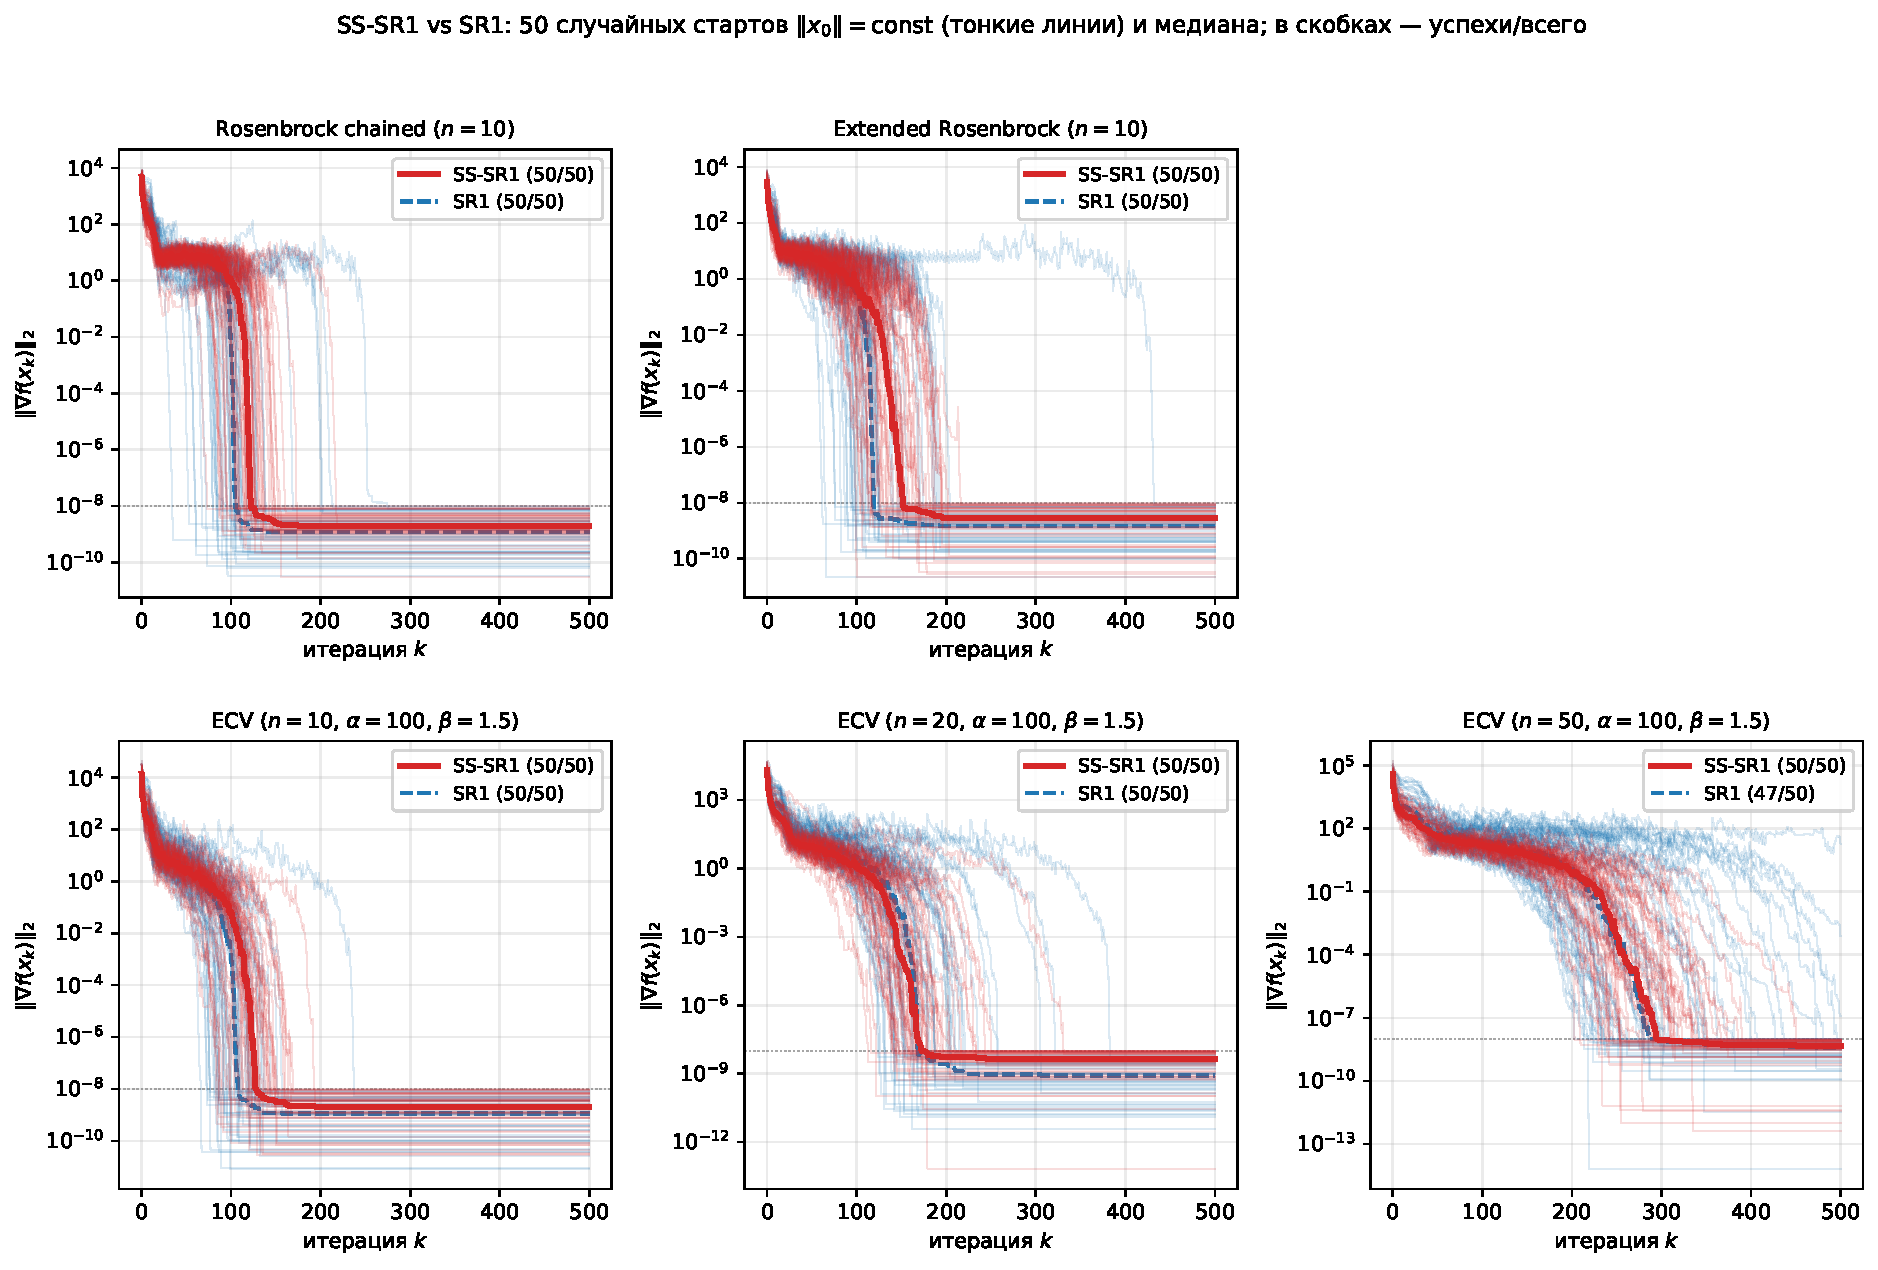
\includegraphics[width=\textwidth]{fig_ndim_stat_sr1.pdf}
\caption{SS-SR1 vs SR1: сходимость $\Norm{\nabla f(x_k)}_2$ на пяти
  тестовых конфигурациях. Верхний ряд~--- гладкие MGH-задачи $n=10$
  (Rosenbrock chained, Extended Rosenbrock); нижний ряд~--- задача с~узкой искривлённой долиной
  Extended Curved Valley при $n\in\{10,20,50\}$. По~$50$~случайных
  стартов на~сфере $\Norm{x_0}=R_0=\Norm{x_0^{\mathrm{std}}}$
  (тонкие линии), медиана жирной линией. На~гладких задачах SS-SR1
  в~медиане на~$15$--$28\,\%$ медленнее~SR1 (накладная стоимость
  MS-коррекции); на~ECV оба метода демонстрируют устойчивую сходимость.}
\label{fig:ndim_stat_sr1}
\end{figure}


% ============================================================
\begin{figure}[htbp]
\centering
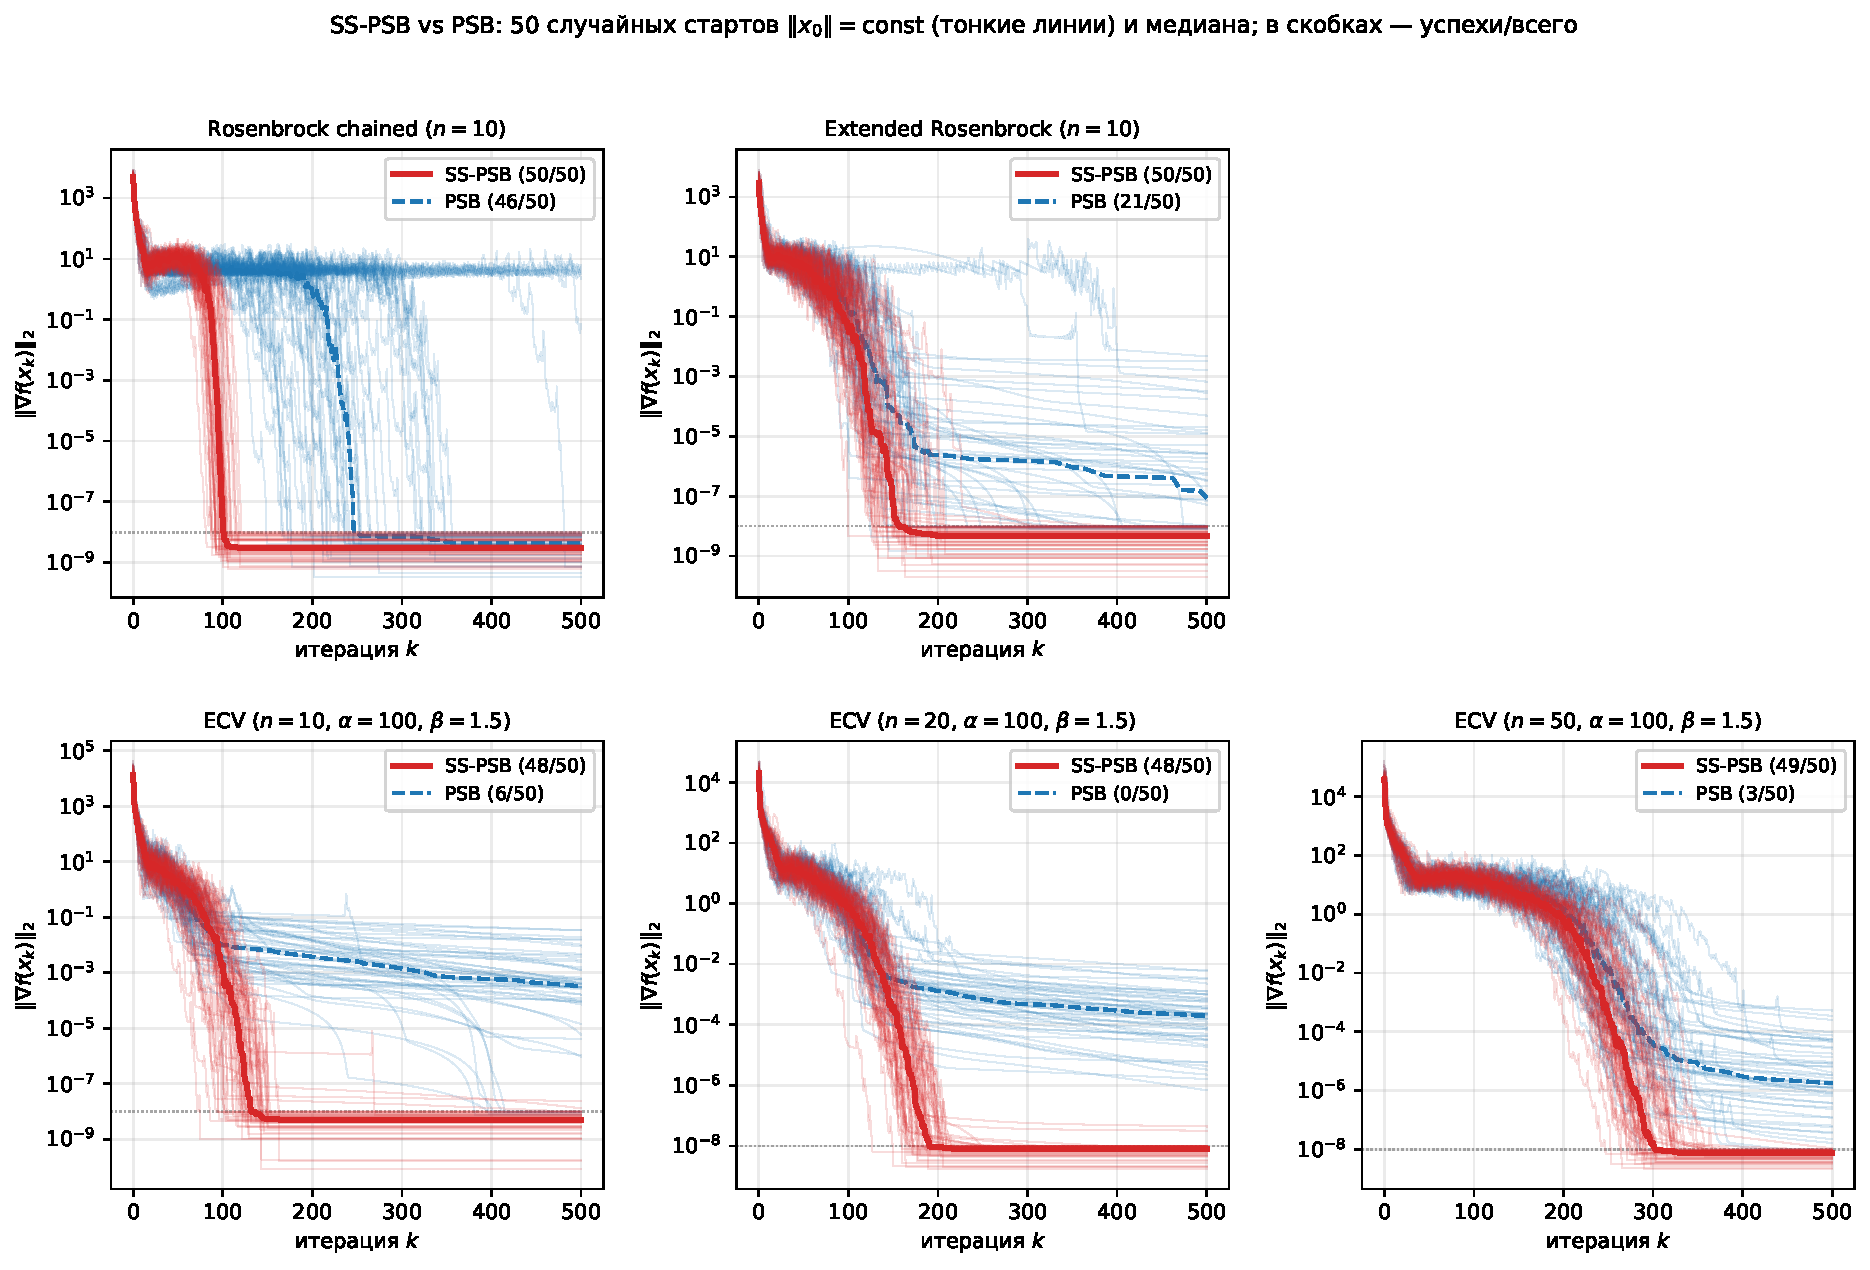
\includegraphics[width=\textwidth]{fig_ndim_stat_psb.pdf}
\caption{SS-PSB vs PSB: те~же пять конфигураций, что на~рис.~\ref{fig:ndim_stat_sr1}.
  Чистый~PSB деградирует уже на~гладких MGH-задачах и~практически
  не~сходится на~ECV; SS-PSB обеспечивает устойчивую сходимость
  на~всех конфигурациях и~на~гладких задачах обходит~PSB по~медиане
  числа итераций. Иллюстрация того, что MS-коррекция способна спасать
  индефинитные базовые обновления с~сильной деградацией.}
\label{fig:ndim_stat_psb}
\end{figure}


% ============================================================
\paragraph{Прямая иллюстрация теоремы~\ref{thm:ss_props}, п.~3:
  динамика накопленной невязки на паре PSB\,/\,SS-PSB.}\label{par:ssn-rpast}
Convergence-кривые рис.~\ref{fig:ndim_stat_sr1}
и~\ref{fig:ndim_stat_psb} показывают итоговую долю сходимости
и~медианное число итераций, но~оставляют открытым прямой
вопрос: действительно ли MS-коррекция \emph{ограничивает} накопленную
невязку $\Norm{B_k S_p - Y_p}_F$ в~смысле теоремы~\ref{thm:ss_props}, п.~3?
Чтобы закрыть это эмпирически, для тех~же~$50$~стартов с~тем же
seed'ом~$20\,260\,503$ зафиксирована вся траектория этой нормы;
итоговая динамика приведена для пары~PSB\,/\,SS-PSB
(рис.~\ref{fig:ndim_stat_rpast_psb}; медиана жирной линией,
заливка~--- межквартильный размах $q_{25}$--$q_{75}$ по~$50$~стартам;
расходящиеся траектории включены через pad-by-last).

Пара PSB\,/\,SS-PSB выбрана как чистая иллюстрация по~двум причинам.
Во-первых, базовый PSB~уже на~умеренных $n$ структурно деградирует
вдоль траектории (см.\ рис.~\ref{fig:ndim_stat_psb}); это даёт
MS-коррекции достаточно \emph{материала}~для работы и~делает разрыв
$\Norm{B_k S_p - Y_p}_F$ визуально разрешимым. Во-вторых, для пары
SR1\,/\,SS-SR1 базовый~SR1 на~использованных режимах часто и~без
MS-коррекции удерживает $\Norm{B_k S_p - Y_p}_F$ на~приемлемом
уровне (что отражает ограничение самой теоремы~Th.~\ref{thm:ss_dm}:
MS-коррекция нужна там, где~SR1 \emph{реально}~деградирует, и~не
создаёт преимущества там, где уже не~деградирует), так что~прямая
rpast-картинка для этой пары читается хуже, чем косвенная сходимостная
метрика рис.~\ref{fig:ndim_stat_sr1}; пара оставлена иллюстрироваться
через~convergence на~рис.~\ref{fig:ndim_stat_sr1}.

Картина на~рис.~\ref{fig:ndim_stat_rpast_psb} согласуется
со~структурным предсказанием. На~всех пяти конфигурациях
SS-PSB снижает медиану $\Norm{B_k S_p - Y_p}_F$ на~$3$--$5$~порядков
относительно~PSB. Особенно показателен режим~ECV, в~котором PSB
теряет устойчивость: $\Norm{B_k S_p - Y_p}_F$ у~него остаётся
выше $10^{-3}$, тогда как~SS-PSB планомерно снижает её до~$\sim 10^{-7}$.
Это прямая эмпирическая поддержка утверждения~3~теоремы~\ref{thm:ss_props}:
оценка
$\Norm{R_{\mathrm{past}}^{(k+1)}}_F^2 \le \Norm{R'_{\mathrm{past}}}_F^2 -
(u_k^{*\top} M'_k u_k^*)^2/\Norm{S_p^{\top} u_k^*}^2$
выполнена по~построению на~каждом шаге; интегральный эффект~---
системно меньшая медиана $\Norm{B_k S_p - Y_p}_F$~--- наблюдается
именно там, где базовое обновление действительно теряет устойчивость.

\begin{figure}[htbp]
\centering
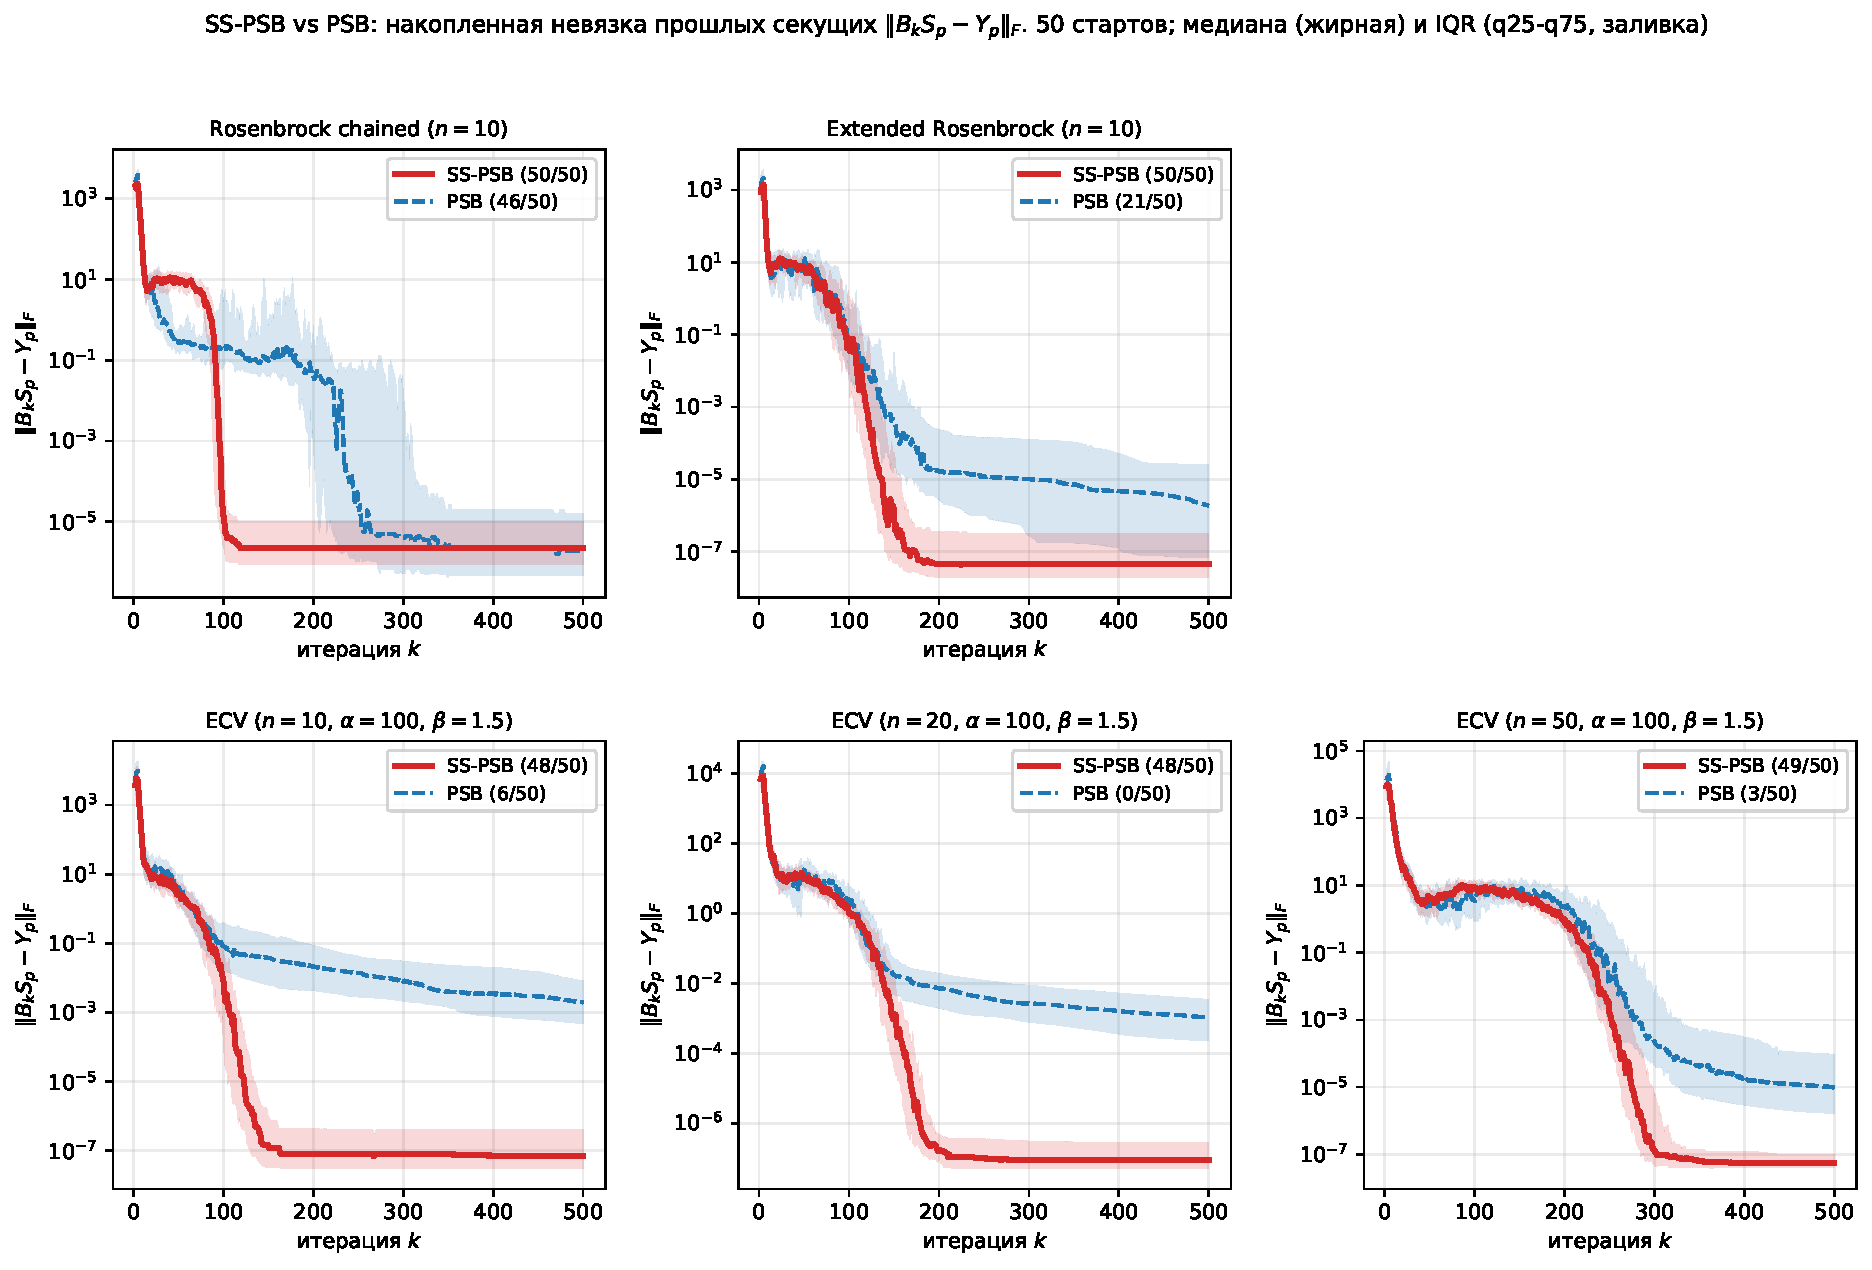
\includegraphics[width=\textwidth]{fig_ndim_stat_rpast_psb.pdf}
\caption{Накопленная невязка прошлых секущих
  $\Norm{B_k S_p - Y_p}_F$ для пары~PSB\,/\,SS-PSB на~тех же~пяти
  конфигурациях, что и~рис.~\ref{fig:ndim_stat_psb}; медиана по~$50$~стартам
  (жирная линия) и~межквартильный размах~q$_{25}$--q$_{75}$ (заливка).
  Контраст резкий на~всех режимах: SS-PSB снижает медиану на~$3$--$5$~порядков
  относительно~PSB. На~ECV~PSB теряет устойчивость, а~$\Norm{B_k S_p - Y_p}_F$
  у~него остаётся выше $10^{-3}$~--- структурная причина отказа
  базового обновления, против которой и~работает~MS-коррекция.
  Прямая эмпирическая поддержка теоремы~\ref{thm:ss_props}, п.~3.}
\label{fig:ndim_stat_rpast_psb}
\end{figure}


% ============================================================
\paragraph{Сводный вывод.}\label{par:ssn-summary}
SS-конструкция Опр.~\ref{def:ss} имеет ясную область применимости~---
индефинитные базовые обновления, у~которых $B_k$ структурно может
терять полезные спектральные свойства.
На~двух таких базовых обновлениях~--- SR1 и~PSB~--- MS-коррекция
эмпирически подтверждает свою роль ограничителя накопленной
невязки $\Norm{B_k S_p - Y_p}_F$ (теорема~\ref{thm:ss_props}, п.~3):
рис.~\ref{fig:ndim_stat_rpast_psb}~--- медиана $\Norm{B_k S_p - Y_p}_F$
у~SS-PSB системно ниже~PSB на~$3$--$5$~порядков, на~ECV~$n=20$ PSB не~сходится,
а~SS-PSB~планомерно снижает невязку до~$\sim 10^{-7}$. Это закрывает
вопрос о~корректности обобщения SS-конструкции на~произвольную
размерность, поставленный в~\S\ref{sec:ss_construction}: ограниченность
$\Norm{B_kS_p-Y_p}_F$ на~всём окне~--- именно тот эффект, который
MS-коррекция должна давать по~построению.


